\documentclass[serif,mathserif]{beamer}
\usepackage{amsmath, amsfonts, epsfig, xspace}
\usepackage{algorithm,algorithmic}
\usepackage{pstricks,pst-node}
\usepackage{multimedia}
\usepackage[normal,tight,center]{subfigure}
\setlength{\subfigcapskip}{-.5em}
\usepackage{beamerthemesplit}
\usetheme{lankton-keynote}

\author[Raptor WAF v0.3]{ Raptor Web Application Firewall \quad 
\includegraphics[width=2.5cm]{images/raptor2.png} }

\title[ Page \hspace{2em}\insertframenumber/\inserttotalframenumber]{Raptor Waf}

\date{November 12, 2015} 

\institute{Antonio Costa - CoolerVoid - coolerlair[aT]gmail[DOt]com}

\begin{document}

\maketitle

% \section{Introduction}  % add these to see outline in slides


\begin{frame}
  \frametitle{Whoami}
  Author:
  \begin{itemize}  \item Antonio Costa "CoolerVoid" is a Computer Programmer who loves the Hacker culture, he work as a system analyst at CONVISO for four years. Antonio working with code review, pentest and security research with focused on Secure Web Applications and Reverse Engineering. He also has been speaking at in some Brazilian Security Conferences such as YSTS, OWASP Florianopolis and Bsides Sao Paulo.
  \end{itemize}
  \begin{figure}[t]
    \centering
    \subfigure[]{
%    \includegraphics[width=3cm]{figures/naked_leaves/00000240}}
    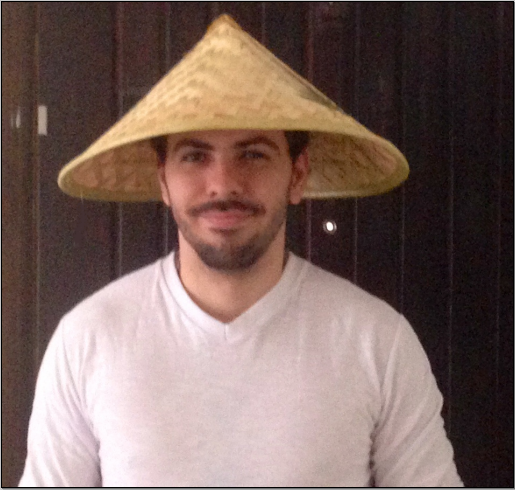
\includegraphics[width=4cm]{images/tony.png}}
  \end{figure}
\end{frame}


\begin{frame}
  \frametitle{Introduction}
  Software Information:
  \begin{itemize}
  \item  Raptor is a Open Source Tool, your focus is study of attacks and find intelligent ways to block attacks. 
  \item  Raptor held by GPL v3 license
  \end{itemize}
\end{frame}



\begin{frame}
  \frametitle{Introduction}
  Why this tool is made in C language ?
  \begin{itemize}
  \item  C have a high delay time for writing and debugging, but no pain no gain, have a fast performance, addition of this point, the C language is run at any architecture like Mips,ARM and others... other benefits of C,  have good and high profile to write optimizations, if you think write some lines in ASSEMBLY code with AES-NI or SiMD instructions, i think is good choice. 
  \item  Why you not use POO ? in this project i follow "KISS" principe: http://pt.wikipedia.org/wiki/Keep\_It\_Simple
  \item  C language have a lot old school dudes like a kernel hackers... 
  \end{itemize}
\end{frame}



\begin{frame}
  \frametitle{Introduction}
  Requirements:
  \begin{itemize}
  \item  Need "GCC" and "make" 
  \item  Current version tested only in Linux.
  \item  Current version run well, but is a BeTa version, you can report bug...
  \end{itemize}
\end{frame}

% \section{Main Body} % add these to see outline in slides

\begin{frame}
  \frametitle{How you can use it}
  Following this to get, decompress, compile and execute:
  \begin{itemize}
  \item wget git clone https://github.com/CoolerVoid/raptor\_waf
  \item cd raptor\_waf; make; bin/Raptor
  \end{itemize}
\end{frame}



\begin{frame}
  \frametitle{The Overview}
  \begin{figure}[]    
    \centering
    
\includegraphics[width=9cm]{images/raptormenu.png} 
  \end{figure}
\end{frame}


\begin{frame}
  \frametitle{Explain}
  WAF stands for Web Application Firewall. It is widely used nowadays to detect and defend SQL Injections and XSS...
  \begin{itemize}
  \item You can block XSS, SQL injection attacks and path traversal with Raptor
  \item You can use blacklist of IPs to block some users at config/blacklist\_ip.txt
  \item You can use IPv6 and IPv4 at communications
  \item At the future DoS protector, request limit, rule interpreter and Malware detector at uploads.
  \item At the future SSL/TLS...
  \end{itemize}
\end{frame}

\begin{frame}
  \frametitle{Hands On !}
  \begin{itemize}
  \begin{figure}[]    
    \centering
    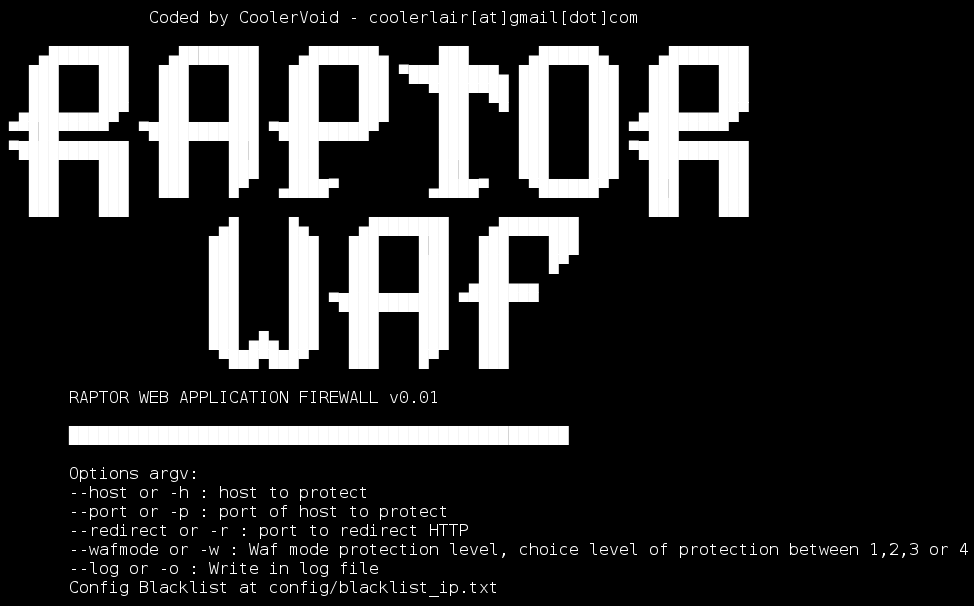
\includegraphics[width=9cm]{images/help.png} 
  \end{figure}
  \end{itemize}
\end{frame}

\begin{frame}
  \frametitle{Hands On !}
  \begin{itemize}
  \item Follow this command
  \item bin/Raptor --host Address\_of\_http\_server2Protect -p 80 -r 8886 -w 4 -o logAttacks.txt 
  \item Open the machine of Raptor at any computer of network http://waf\_machine:8886
  \item Copy vulnerable PHP code to your web server directory
  \item cp doc/test\_dfa/test.php /var/www/html
  \item Ok raptor protect the HTTP server at http://server\_ip:8886/test.php
  \end{itemize}
\end{frame}

\begin{frame}
  \frametitle{How it works ?}
   Raptor is very simple, have three layers reverse proxy, blacklist and Match(using deterministic finite automaton).
  \begin{itemize} 
  \begin{figure}[]    
    \centering
    
\includegraphics[width=8cm]{images/raptor2.png} 
  \end{figure}
  \end{itemize}
\end{frame}



\begin{frame}
  \frametitle{How proxy works ?}
  Proxy using the select() function to check multiple sockets, at the future change to use libevent(signal based is very fast)  
  \begin{itemize} 
  \begin{figure}[]    
    \centering
    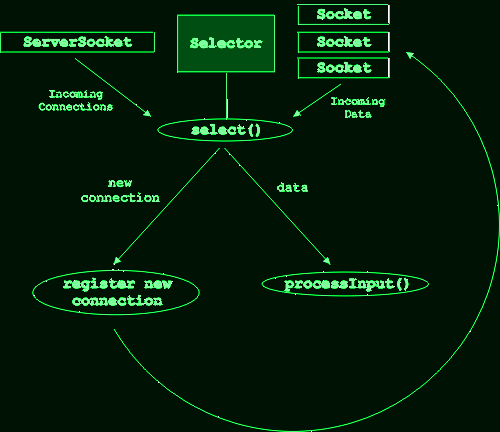
\includegraphics[width=8cm]{images/select.png} 
  \end{figure}
  \end{itemize}
\end{frame}


\begin{frame}
  \frametitle{How it works ?}
  If someone send a request, Raptor do address analysis... Address blacklisted ? block !
  \begin{itemize} 
  \begin{figure}[]    
    \centering
    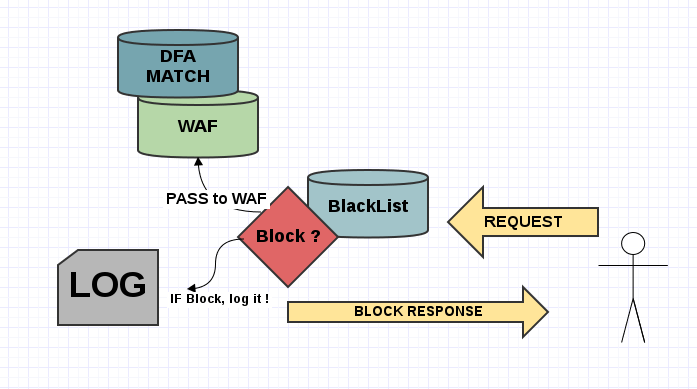
\includegraphics[width=10cm]{images/blockip.png} 
  \end{figure}
  \end{itemize}
\end{frame}

\begin{frame}
  \frametitle{How it works ?}
  If deterministic finite automaton and Blacklist don't match, Raptor don't block 
  \begin{itemize} 
  \begin{figure}[]    
    \centering
    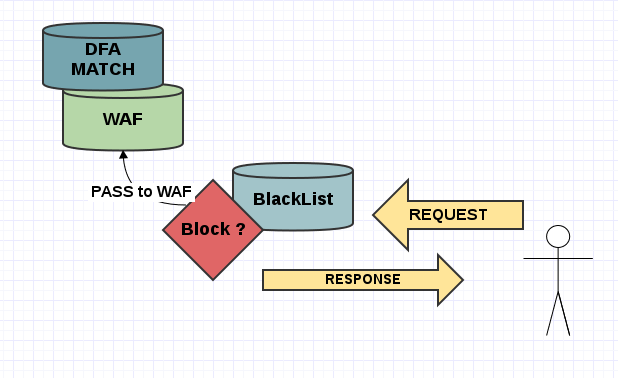
\includegraphics[width=10cm]{images/pass.png} 
  \end{figure}
  \end{itemize}
\end{frame}

\begin{frame}
  \frametitle{How it works ?}
  Raptor get a Request with GET or POST method and make some analysis to find dirt like a sql injection, cross site scripting...
  \begin{itemize} 
  \begin{figure}[]    
    \centering
    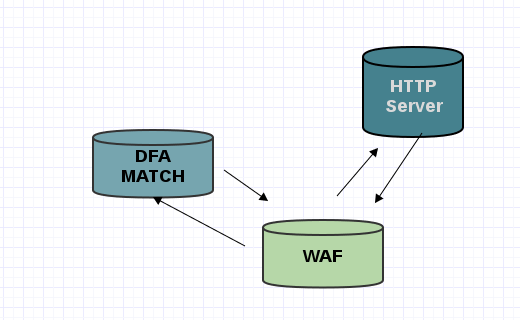
\includegraphics[width=8cm]{images/http.png} 
  \end{figure}
  \end{itemize}
\end{frame}

\begin{frame}
  \frametitle{External match string mode}
  \begin{itemize}
  \item At directory config have a file of lists of rules
  \item You can match string with diferent algorithms
  \item You can choice with argument --match or -m
  \item Choice one option between Karpe Rabin, DFA or Boyer Moore Horspool
  \end{itemize}
\end{frame}

\begin{frame}
  \frametitle{The End ?}
  \begin{figure}[]    
    \centering
    
\includegraphics[width=5cm]{images/raptor0.jpg} 
  \end{figure}
\end{frame}



% \section{Conclusion} % add these to see outline in slides

\begin{frame}
  \frametitle{Greets}
  \begin{itemize}
  \item contact: coolerlair[at]gmail[dot]com 
  \item acosta@conviso.com.br
  \item my parents and friends...
  \item https://conviso.com.br/index.php/EN
  \end{itemize}
\end{frame}

\begin{frame}
  \frametitle{at construction...}
\end{frame}

\end{document}

